\section{Основная часть}
\subsection{Датасет CIFAR-10}
Набор данных, на котором проводились исследования, состоит из 60\,000 цветных изображений, размера 
32$\times$32 пикселя. Каждое изображение принадлежит одному из 10 классов, что соответствует 600 изображениям на класс. Под 
обучение отводится 50\,000 изображений. Остальные 10\,000 используются для тестирования. Объекты в классах сильно варьируются, 
например, класс <<птица>> содержит различные виды птиц, как большие так и маленькие. Кроме того, объекты классов представлены в 
различных позах и под различными углами. Особенно это проявляется среди собак и котов, которые изображены не только в различных 
позах, но иногда и частично, например, изображена только голова животного.

Датасет CIFAR-10 был выбран для проведения исследований благодаря своему относительно небольшому размеру, который позволяет 
обучать глубокие нейронные сети используя GPU с памятью меньше 8\,Gb, например, в данном работе использовалась NVIDIA Grid K520 с 
4\,Gb видеопамяти.

На момент написания работы лучший результат (state-of-the-art) на CIFAR-10 составляет 96.53\% \cite{2014arXiv1412}. Точность 
распознавания человека приблизительно равна 94\% \cite{karpathycifar}.

\begin{figure}[h]
\centering
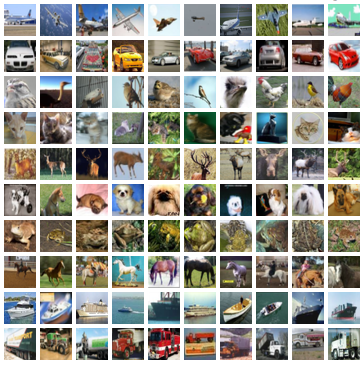
\includegraphics[width=0.5\textwidth]{cifar10}
\caption{10 случайных изображений из каждого класса CIFAR-10}
\end{figure}

\subsection{Фреймворк Caffe}
\subsection{Предварительная обработка данных}
\subsection{Обучение нейронных сетей}
\subsection{Анализ результатов одиночных моделей}
\subsection{Объединение нейронных сетей в ансамбль}